\begin{comment}
\end{comment}

\chapter{Échantillonnage quasi uniforme et comptage approximatif randomisé}

\begin{comment}
\subsection*{Plan}

\begin{enumerate}
    \item Énoncer brièvement l'algorithme de JVV pour introduire la section
    \item Re-mentionner l'importance du comptage approximatif (en autres en comparaison avec le comptage exact)
    \item Mentionner les concepts nécessaires pour l'algorithme de JVV (auto-réductibilité, échantillonnage quasi aléatoire, comptage approximatif)
\end{enumerate}
\subsection*{Références}
\end{comment}

Dans une publication marquante pour le domaine de la complexité du comptage, Jerrum, Valiant et Vazirani ont montré que l'échantillonage quasi uniforme de structures combinatoriales est d'une complexité équivalente au comptage approximatif randomisé~\cite{jerrumRandomGenerationCombinatorial1986}. Un algorithme de comptage approximatif utilise cette correspondance pour résoudre approximativement les problèmes de comptage auto-réductibles avec un générateur de solution quasi uniforme.

Les trois concepts nécessaires à l'algorithme de JVV sont présentés dans cette section: l'auto-réductibilité, l'échantillonnage quasi-uniforme et le comptage approximatif.

Une \textit{structure combinatoriale} se définit comme un système discret fini comportant des éléments et des relations bien définies. Par exemple, une formule propositionnelle, composée de variables booléennes et de contraintes sous forme d'opérateurs booléens, est associée à un ensemble discret de solutions.

Dans la section précédente, les problème de décision, ou équivalemment d'existence, et de comptage ont été introduit. Ces problèmes se cadrent à l'intérieur d'autre types de problèmes: 

\begin{enumerate}[(1)]
    \item \textbf{Existence}: Existe-t-il une solution au problème?
    \item \textbf{Construction}: Construire une solution au problème.
    \item \textbf{Génération uniforme}: Générer uniformément et aléatoirement une solution au problème.
    \item \textbf{Comptage} Combien de solutions satisfont le problème?
\end{enumerate}




\textcolor{mydarkred}{\textit{Rajouter une citation au papier de JVV.}}

%-----------------------------------------------------------------------------%

\section{Auto-réductibilité}
\label{sec:auto-reductibilite}
 
\begin{comment}
\subsection*{Plan}

\begin{enumerate}
    \item Introduire les concepts d'auto-réductibilité
\end{enumerate}

\subsection*{Références}

1. Hemaspaandra, L. A. The Power of Self-Reducibility: Selectivity, Information, and Approximation. Preprint at https://doi.org/10.48550/arXiv.1902.08299 (2019).

\subsection*{Brouillon}

Introduction de "Autoreducibility" par Trakhtenbrot.

Introduction de "Self-reducibility" par Schnorr et Meyer/Paterson.

Survey paper de Balcázar, Selke, Allender.

Explication simple par Hemaspaandra.
\end{comment}

L'\textit{auto-réductibilité} (« self-reducibility ») est un concept complexe, essentiel à la compréhension du calcul et de la complexité, découlant de l'introduction de la \textit{réduction automatique} (« autoreducibility »)~\cite{trakhtenbrotAutoreducibility1970}. Ces concepts sont particulièrement importants dans le contexte de génération aléatoire et du comptage approximatif, ainsi que pour la réduction entre le problème de décision et les problèmes de recherche.

La \textit{réduction automatique} peut être introduite informellement de la manière suivante:

\begin{subdefinition}{Réduction automatique}{auto-reductibilite}
    Un problème algorithmique est dit \textit{automatiquement réductible} s'il peut être résolu par un algorithme résolvant d'autres instances du même problème, sans que l'algorithme puisse interroger l'instance particulière qu'il cherche à résoudre.
\end{subdefinition}

Les problèmes automatiquement réductibles contiennent de l'information d'appartenance redondante, c'est-à-dire qu'il existe une structure dans l'ensemble de problèmes pouvant être exploitée pour simplifier le calcul d'une instance donnée. Ainsi, un algorithme peut résoudre une instance en utilisant l'information redondante présente dans d'autres instances, évitant ainsi les requêtes directes à l'instance en question. Connaître la solution à une autre problème peut alors aider la résolution du problème initial. 

\textcolor{mydarkred}{\textit{Exemple: Halting problem?}}

Pour discuter de la génération aléatoire et le comptage approximatif, l'\textit{auto-réductibilité descendante}, une forme limité de la réduction automatique, est une définition plus adéquate. En effet, cette condition est nécessaire à l'application de l'algorithme JVV. Informellement, on peut définir celle-ci comme:

\begin{maindefinition}{Auto-réductibilité descendante}{auto-reductibilite-informel}
    Un problème algorithmique est dit \textit{auto-réductible descendant} s'il peut être résolu grâce à un algorithme résolvant des instances de taille strictement inférieure.
\end{maindefinition}

\textcolor{mydarkred}{\textit{Quelle est vraiment la différence entre auto-reducibility et self-reducibility?}}

Cette propriété s'éclaircit en prenant le problème SAT comme exemple, qui s'avéra particulièrement utile dans la compréhension de l'algorithme JVV à la section~\ref{sec:algorithme-jvv}. L'auto-réductibilité appliquée au problème de satisfaisabilité s'exprime facilement avec la relation suivante:

\begin{relation}{Auto-réductibilité pour les problèmes SAT}{auto-reductibilite-sat}
    Soit une constante $n \geq 1$ et une formule propositionelle $\varphi(x_{1}, x_{2}, \dots, x_{n})$ où $x_{i} \in \set{ 0, 1 }$. Alors,
    \begin{equation*}
        \varphi(x_{1}, x_{2}, \dots, x_{n}) = 1 \iff \varphi(x_{1}=0, x_{2}, \dots, x_{n}) = 1 \lor \varphi(x_{1}=1, x_{2}, \dots, x_{n}) = 1
    \end{equation*}
\end{relation}

Cette relation implique que l'ensemble de solutions d'une instance donnée peut être exprimée comme l'ensemble de solutions de deux instances plus petites du problème. Supposons que l'on souhaite résoudre une instance du problème SAT décrit par la formule CNF $\varphi(x_{1}, x_{2}, \dots, x_{n})$. Soit $\varphi_{0} = \varphi(x_{1}=0, \dots, x_{n})$ et $\varphi_{1} = \varphi(x_{1}=1, \dots, x_{n})$ deux sous-instances de l'instance $\varphi$, où la variable $x_{1}$ est remplacée par 0 et 1 respectivement. Se faisant, la formule $\varphi$ est alors raccourcie, comme certaines clauses sont satisfaits ou du moins réduites. Pour que l'instance $\varphi$ soit satisfaisable, il est alors nécessaire qu'au moins une des sous-instances $\varphi_{0}$ et $\varphi_{1}$ soit satisfaible. Dans le cas contraire, l'instance originale $\varphi$ ne peut être satisfaible car il n'existe pas de solution peu importe la valeur de $x_{1}$. Ainsi, il suffit de considérer la disjonction des sous-problèmes possibles du problème original pour résoudre ce dernier. Les sous-problèmes obtenus étant aussi des formules propositionnelles, ceux-ci peuvent aussi être décomposés en problème de taille inférieure récursivement jusqu'à obtenir un problème complètement fixé. Notons de plus qu'il n'est pas nécessaire de construire la relation~\ref{rel:auto-reductibilite-sat} avec la variable $x_{1}$, n'importe quelle variable $x_{i}$ peut aussi être utilisée.

Plus précisément, le problème SAT est décrit comme une auto-réductibilité à longueur décroissante 2-disjonctive. Ici, 2-disjonctive fait référence à une formule propositionnelle dans une disjonction ($\lor$) d'une conjonction ($\land$) d'au plus deux variables. Longueur décroissante, ou descendante, signifie que l'algorithme résout des instances de taille strictement inférieure.

L'auto-réductibilité est simplement généralisable aux problèmes dont les variables peuvent prendre un plus grand nombre de valeurs en prennant la disjonction sur toutes les valeurs possibles.

\textcolor{mydarkred}{\textit{Élaborer...}}

La relation~\ref{rel:auto-reductibilite-sat} exemplifie une deuxième façon de voir l'auto-réductibilité: la résolution partielle d'une instance d'un problème laisse une plus petite instance du même type de problème. Une autre manière de l'interprêter est qu'une instance peut être résolue en résolvant des plus petites instances et en assemblant les sous-instances ensemble.

\textcolor{mydarkred}{\textit{Exemple: casse-tête}}

Afin d'obtenir une meilleure perspective sur la notion d'auto-réductibilité, il est pertinent d'exprimer la structure d'une relation auto-réductible $\varphi$ sous la forme d'un arbre orienté, nommé \textit{arbre d'auto-réductibilité}. Dans cet arbre, les sommets représentent à la fois une chaîne de bits $w$ de taille $m$ et une instance de problème $\varphi_{w}$, où $\varphi_{w}$ représente la sous-instance du problème $\varphi$ dont les premières variables sont remplacées par la chaîne de bits $w$. Le sous-problème est alors dit \textit{fixé} par la le préfixe $w$. La racine de l'arbre correspond à l'instance du problème initial $\varphi$ ainsi qu'à une solution partielle nulle. Par la suite, les enfants de cette racine sont donnés par les sous-instances $\varphi_{w}$ pour tous les préfixes $w$ de taille $1$ possibles. Le reste de l'arbre est alors défini récursivement de la même manière en augmentant la taille de la chaîne de bits $w$ à chaque niveau jusqu'aux feuilles de l'arbre. Ces feuilles représentent alors une solution au problème $\varphi$.

Le degrée de l'arbre est donné par le nombre de valeurs que peut prendre une variable. Dans le cas du problème SAT, les variables sont booléennes et donc le degré de l'arbre est de deux.

La figure \textcolor{mydarkred}{\textit{Ajouter la figure.}}

Notons que l'arbre d'auto-réductibilité est aussi parfois défini tel les feuilles correspondent uniquement à des solutions au problème auto-réductible. Ainsi, les ramifications de l'arbre ne comprennent pas les non-solutions.

Une définition rigoureuse de l'auto-réductibilité peut aussi être pratique.

\begin{maindefinition}{Auto-réductibilité descendante}{auto-reductibilite-formel}
    Soit $\Sigma^{*}$ un ensemble fixé et fini encodant les instances d'un problème ainsi que leurs solutions. Soit $R \subseteq \Sigma^{*} \times \Sigma^{*}$ une relation binaire assignant à chaque instance de problème $x \in \Sigma^{*}$ un ensemble de solutions $R(x) = \set{ y \in \Sigma^{*} \mid xRy }$. Une relation $R \subseteq \Sigma^{*} \times \Sigma^{*}$ est auto-réductible si et seulement si
    \begin{enumerate}
        \item il existe une fonction calculable en temps polynomial $g \in \sigma^{*} \to \mathbb{N}$ tel que $xRy \implies \lvert y \rvert = g(x)$;
        \item il existe une fonction calculable en temps polynomial $\psi \in \Sigma^{*} \times \Sigma^{*} \to \Sigma^{*}$ et $\sigma \in \Sigma^{*} \to \mathbb{N}$ satifaisant
        \begin{align*}
            & \sigma(x)=O(\log |x|) \\
            & g(x)>0 \Rightarrow \sigma(x)>0 \quad \forall x \in \Sigma^{\star} \\
            & |\psi(x, w)| \leqslant|x| \quad \forall x, w \in \Sigma^{\star}
        \end{align*}
        et tel que, pour tout $x \in \Sigma^{*}, y=y_1 \ldots y_n \in \Sigma^{*}$, 
        \begin{equation*}
            \left\langle x, y_1 \ldots y_n \right\rangle \in R \Leftrightarrow \left\langle \psi \left( x, y_1 \ldots, y_{\sigma(x)} \right), y_{\sigma(x)+1} \ldots y_n \right\rangle \in R
        \end{equation*}
    \end{enumerate}
\end{maindefinition}

Notons que la définition de l'auto-réducibilité utilisée dans cette section s'applique principalement à l'équivalence entre l'échantillonnage quasi uniforme et le comptage approximatif randomisé. Cependant, une définition alternative~\cite{goldreichComputationalComplexityConceptual2008a} est souvent introduite pour l'équivalence entre les problèmes de décision et les problèmes de recherche, où un problème de recherche ne demande pas de montrer l'existence d'une solution, mais de construire une telle solution. En effet, si un problème est auto-réductible dans ce sens, alors le problème de décision est de la même complexité que le problème de recherche. 

\textcolor{mydarkred}{\textit{Parler du lien avec les problème de recherche.}}

\textcolor{mydarkred}{\textit{Most of NP problems exhibit self-reducibility.}}

%-----------------------------------------------------------------------------%

\section{Échantillonnage quasi uniforme}

\begin{comment}
\subsection*{Plan}

\begin{enumerate}
    \item Introduire les FPAUS
    \item Introduire la distance en variation totale et la non-uniformité
\end{enumerate}

\subsection*{Références}
\end{comment}

\textcolor{mydarkred}{\textit{L'existence est plus facile que le comptage.}}
\textcolor{mydarkred}{\textit{L'échantillonnage uniforme est plus facile que le comptage.}}


L'échantillonage uniforme étant une demande plutôt rigide, il est parfois nécessaire de relaxer la condition d'uniformité pour une quasi uniformité. Une distribution quasi uniforme est en pratique indifférentiable d'une distribution uniforme, mais ce relâchement facilite les preuves, comme montré à la section~\ref{sec:algorithme-jvv}.

\begin{maindefinition}{Échantillonneur quasi uniforme polynomial~\cite{jerrumCountingSamplingIntegrating2003}}{fpaus}
    Un échantillonneur quasi uniforme pour un ensemble de solutions $S \subseteq \Sigma^{*} \times \Sigma^{*}$, où $S$ représente la relation entre les instances d'un problème $x$ et de ses solutions $y \in  S(x)$, est un algorithme aléatoire prenant en entrée une instance $x \in \Sigma^{*}$ et une tolérance d'échantillonnage $\delta > 0$ et qui génère une solution $y \in S(x)$ tel que
    \begin{equation*}
        \lVert Y - U \rVert_{TV} \leq \delta 
    \end{equation*}
    où $Y$ est la distribution de probabilité de $y$ et $U$ est la distribution de probabilité uniforme sur $S(x)$. Si l'algorithme s'exécute en temps borné par un polynomial en $\lvert x \rvert$ et en $\ln (\delta^{-1})$, on parle d'échantillonneur quasi uniforme pleinement polynomial.
\end{maindefinition}

\textcolor{mydarkred}{\textit{Changer la définition pour celle du papier de JVV? Oui, et décrire le lien avec la TVD.}}

Une définition alternative utilise plutôt la \textit{distance en variation totale}. Cette quantité statistique décrit la distance entre deux distributions de probabilité.

\begin{subdefinition}{Distance en variation totale}{tvd}
    Soit deux distributions de probabilité $P$ et $Q$ définies sur un ensemble $\chi$. La distance en variation totale est
    \begin{equation*}
        \lVert P - Q \rVert_{TV} \equiv \frac{1}{2} \sum_{x \in \chi} \lvert P(x) - Q(x) \rvert \,. 
    \end{equation*}
\end{subdefinition}

Une notion supplémentaire est introduite dans ce mémoire afin de simplifier la notation. La \textit{non-uniformité}, de manière similaire à la distance en variation totale, décrit la distance entre une distribution de probabilité $Q$ et la distribution de probabilité uniforme $U$.

\begin{maindefinition}{Non-uniformité}{non-uniformite}
    Soit la distribution de probabilité $P$ et la distribution de probabilité uniforme $U$ tel que $U(x) = 1/\lvert x \rvert$ définies sur un ensemble $\chi$. La non-uniformité est
    \begin{equation*}
        \eta \equiv \frac{1}{2} \sum_{x \in \chi} \lvert P(x) - U(x) \rvert \,. 
    \end{equation*}
\end{maindefinition}

\textcolor{mydarkred}{\textit{https://page.math.tu-berlin.de/~felsner/Lehre/SemProbMeth/XX-Jerrum.pdf}}


%-----------------------------------------------------------------------------%

\section{Comptage approximatif randomisé}

\begin{comment}
\subsection*{Plan}

\begin{enumerate}
    \item Introduire les FPRAS
    \item Introduire les algorithmes de comptage classique connus (ex.: Stockmeyer et JVV)
\end{enumerate}

\subsection*{Références}

1. Stockmeyer, L. The complexity of approximate counting. in Proceedings of the fifteenth annual ACM symposium on Theory of computing 118–126 (Association for Computing Machinery, New York, NY, USA, 1983). doi:10.1145/800061.808740.
\end{comment}

Un algorithme d'approximation pour le comptage se définit de manière similaire à l'algorithme d'approximation pour l'optimisation décrit à la section~\ref{intractabilite-approximation-et-optimisation}.

\begin{maindefinition}{Schéma d'approximation randomisé polynomial}{fpras}
    Un schéma d'approximation randomisé pour un problème de comptage $f: \Sigma^{*} \to \mathbb{N}$ est un algorithme randomisé prenant en entrée une instance d'un problème $x \in \Sigma^{*}$ et une tolérance d'erreur $\varepsilon > 0$ et qui génère un nombre $N \in \mathbb{N}$ tel que, pour toute instance $x$,
    \begin{equation*}
        \mathrm{ Pr }\left[(1+\varepsilon)^{-1} f(x) \leq N \leq (1+\varepsilon)f(x)\right] \geq \frac{3}{4} .
    \end{equation*}
    Si l'algorithme s'exécute en temps borné par un polynomial en $\lvert x \rvert$ et $\varepsilon^{-1}$, alors on parle de schéma d'approximation aléatoire pleinement polynomial.
\end{maindefinition}

%-----------------------------------------------------------------------------%

\section{Algorithme de Jerrum-Valiant-Vazirani}
\label{sec:algorithme-jvv}

\begin{comment}
\subsection*{Plan}

\begin{enumerate}
    \item Introduire le but de l'algorithme de JVV
    \item Vulgariser l'algorithme de JVV
    \item Introduire rigoureusement l'algorithme de JVV
    \item Rajouter l'algorithme complet sous forme de pseudo-code.
\end{enumerate}

\subsection*{Références}

1. Jerrum, M. R., Valiant, L. G. and Vazirani, V. V. Random generation of combinatorial structures from a uniform distribution. Theoretical Computer Science 43, 169–188 (1986).
2. Huber, M. Exact sampling and approximate counting techniques. in Proceedings of the thirtieth annual ACM symposium on Theory of computing 31–40 (Association for Computing Machinery, New York, NY, USA, 1998). doi:10.1145/276698.276709.
\end{comment}


Le travail de Jerrum, Valiant et Vazirani~\cite{jerrumRandomGenerationCombinatorial1986} se poursuit en établissant une correspondance entre l'échantillonnage quasi uniforme et le comptage approximatif randomisé. Pour ce faire, deux algorithmes permettant le passage d'un problème à l'autre sont présentés. Bien la réduction du comptage à l'échantillonage est intéressante, elle ne sera discuté que brièvement à la fin de la section comme la réduction d'importance est ici son inverse. L'algorithme de comptage approximatif randomisé, nommé \textit{algorithme de JVV} selon le nom de ses auteurs, permet de trouver le nombre de solutions d'un problème auto-réductible de la classe \textsf{\#P} à une erreur multiplicative près en utilisant un générateur de solution quasi uniforme. 

\textcolor{mydarkred}{\textit{Expliquer le lien entre les deux concepts et les preuves.}}

\begin{maintheorem}{Algorithme de JVV}{algorithme-jvv}
    Si un problème algorithmique auto-réductible dans \textsf{\#P} de taille $n$ admet un générateur de solutions avec une non-uniformité $\eta = O(\varepsilon / n)$, alors le nombre de solutions peut être approximé à une erreur multiplicative de $\varepsilon$ avec une haute probabilité avec $O(n^{2}/\varepsilon^{2})$ appels au générateur.
\end{maintheorem}

Comment est-ce que l'algorithme de JVV opère? Commençons par introduire l'idée principale derrière l'algorithme, pour ensuite donner un exemple simple, et compléter avec une description plus mathématique. 

Pour mieux comprendre son exécution, l'arbre d'auto-réductibilité, présenté à la section~\ref{sec:auto-reductibilite}, sera utilisé. L'algorithme de JVV implique de marcher vers le haut ou vers le bas de cet arbre, en s'intéressant à tous les sous-instances en chemin.

Démontrons d'abord comment compter approximativement en utilisant un générateur uniforme de solutions. Supposons qu'il est possible d'échantilloner uniformément les solutions de n'importe quelle instance du problème SAT. D'abord, des solutions au problème initial $\varphi$, représenté par racine de l'arbre, sont échantillonnées. Soit $P_{0}$ et $P_{1}$ les probabilités que la variable $x_{1}$ soit respectivement de 0 et 1 dans les solutions échantillonnés. Ces probabilités réflètent alors la proportion de solutions dans chaque sous-arbre. Par la suite, nous descendons l'arbre vers l'enfant le plus probable $w_{0}$, en gardant en mémoire la probabilité $P_{w_{0}}$. Comme notre échantillonneur peut aussi résoudre le problème subséquent, nous pouvons encore déterminer quelle variable est la plus probable en déterminant la probabilité $P_{w_{1}}$. Le processus est répété jusqu'à atteindre les feuilles de l'arbre, en sauvegardant les probabilités $P_{w}$ le long du chemin choisi $w$. Au dernier noeud avant les feuilles, une solution est obtenue avec une probabilité $P_{w_{n}}$. Comme nous sommes à la base de l'arbre, cette probabilité indique le nombre de solutions associées à la dernière sous-instance. Alors, ce sous-arbre contient nécessairement $\frac{1}{P_{w_{n}}}$ solutions, car il y a soit aucune, une ou deux solutions dans la dernière sous-instance. En remontant l'arbre, on remarque que la sous-instance précédente contient $\frac{1}{P_{w_{n-1}}}$ fois plus de solutions. Par conséquent, le nombre de solutions dans cette partie de l'arbre est de $\frac{1}{P_{w_{n}}} \frac{1}{P_{w_{n-1}}}$. Continuant cette procédure jusqu'à la racine, nous trouvons que le nombre de solutions est donné par 


\begin{equation}
    N = \frac{1}{P_{w_{0}}} \frac{1}{P_{w_{m}}} \dots \frac{1}{P_{w_{n}}} = \frac{N}{N_{w_{0}}} \frac{N_{w_{0}}}{N_{w_{1}}} \dots \frac{N_{w_{n-1}}}{N_{w_{n}}}
\end{equation}

Éclaircissons maintenant l'idée derrière l'algorithme de JVV à l'aide d'un exemple simple tel qu'illustré à la figure~\ref{fig:algorithme-jvv}. Soit une instance du problème SAT décrite par la formule CNF $\varphi(x_{1}, x_{2}) = \neg x_{1} \land x_{2}$, dont les solutions sont les couples $(0,0)$, $(0,1)$ et $(1,1)$. Un arbre est construit de manière à représenter tous les sous-instances de l'instance originale. Chaque niveau de l'arbre correspond à l'attribution d'une valeur, 0 ou 1, à une variable, constituant ainsi une sous-instance du problème initial. La racine de l'arbre représente le problème initial et ses deux variables $x_{1}$ et $x_{2}$. La première couche représente les sous-problèmes $\varphi_{0}$ et $\varphi_{1}$ où la première variable est remplaçée par 0 et 1 respectivement. Dans la dernière couche, les feuilles représentent les assignations possibles au problème $\varphi$, c'est-à-dire lorsque toutes les variables sont fixées à une certaine valeur. À chaque arrête de l'arbre, une probabilité décrit la probabilité qu'une solution au p


\begin{figure}[h]
    \centering
    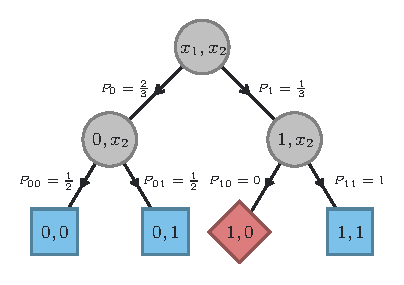
\includegraphics[width=0.55\textwidth]{figures/jvv-algorithm.pdf}
    \caption{}
    \label{fig:algorithme-jvv}
\end{figure}

Supposons que le nombre exact de solutions pour une instance de problème SAT de $n$ est de $N$. 

\begin{align}
    p^\star = \frac1N =&{\ } \frac{N_{z_{:1}}}{N} \cdot \frac{N_{z_{:2}}}{N_{z_{:1}}} \cdots \frac{N_{z_{:n}}}{N_{z_{:n-1}}} \\
    =&{\ } p(z_{:1}) \cdot p(z_{:2}|z_{:1}) \cdots p(z_{:n}|z_{:n-1}) \\
    =&{\ } p(z_{:1}) \prod_{i=1}^{n-1} p(z_{:i+1}|z_{:i}) \,,
\end{align}

\begin{equation}
    \tilde p(z_{:i+1}|z_{:i}) = \frac{ \tilde N_{z_{:i+1}} }{ \tilde N_{z_{:i}} } \,,
\end{equation}

\begin{equation}
    \tilde p^\star = \tilde p(z_{:1}) \prod_{i=1}^{n-1} \tilde p(z_{:i+1}|z_{:i}) \approx \frac1N \,.
\end{equation}

% Les solutions à ce problème sont facilement vérifiable par examination. Le problème SAT étant auto-réductible, un arbre d'auto-réductibilité peut être construit de manière à représenter tous ses sous-problèmes tel qu'illustré à la figure~\ref{fig:algorithme-jvv}. Supposons qu'il soit possible d'estimer 

% Comme décrit à la section~\ref{sec:auto-reductibilite}, chaque noeud de l'arbre est associé une chaîne de bits $w$ de taille $m$ fixant les $m$ premières variables de la formule $\varphi$ ainsi qu'une formule partielle $\varphi_{w}$. 

\textcolor{mydarkred}{\textit{Ajouter un algorithme.}}